\documentclass[a4paper,11pt]{article}

\usepackage[top=1in, bottom=1.25in, left=1.25in, right=1.25in]{geometry}
\usepackage{graphicx}
\usepackage{amsmath}
\usepackage{amssymb}
\usepackage[style=numeric-comp,sorting=none]{biblatex}
\usepackage{warning} % for warning messages

\parskip=1.5ex
\parindent=0pt

\usepackage{url}
\usepackage{microtype}
\usepackage{lmodern}
\usepackage[colorlinks=true, citecolor=red, linkcolor=blue]{hyperref}

\usepackage{caption}
\usepackage{subcaption}
\usepackage{float}
\usepackage{booktabs}
\usepackage{multirow}
\usepackage[affil-it]{authblk}


\usepackage{todonotes}

\usepackage{siunitx}

\usepackage[compat=1.1.0]{tikz-feynman} % generate feynman diagrams

\renewcommand{\vec}{\mathbf}
\newcommand{\ts}{\textsuperscript}

\bibliography{references}
\overfullrule=2cm % allows to find overfull hboxes much quicker

\binoppenalty=3000
\relpenalty=3000

\title{Applications of Standard Model Effective Field Theory to 2D differential distributions of top pair production}
\author{Alexander Veltman\\{\small Advisor: Dr.\ James Keaveney}}
\affil{Department of Physics,\\University of Cape Town}

\begin{document}
\maketitle

\begin{abstract}
\end{abstract}

\section{Introduction}

\begin{itemize}
    \item Standard model is good
    \item Cannot explain some phenomena
    \item New frame work called SMEFT
\end{itemize}


\section{Top Physics}

The top quark is the most massive particle in the Standard Model with a rest mass of $m_{t} =172.76\pm0.30$GeV~\cite{ParticleDataGroup:2020ssz} and is commonly used as an regime to look for physics beyond the Standard Model.
Due to high luminosity achieved by the various experiments present at the Large Hardron Collider, very detailed cross sectional measurements have been achieved, allowing for the ability to implement differential cross section measurements of top quark production in high energy physics analysis.

Top quarks are usually produce in top-antitop pairs through the $gg\rightarrow t\bar{t}$ and $q\bar{q}\rightarrow t\bar{t}$ processes at leading order.
Leading order (LO) and next-to-leading order (NLO) refer to the number of interactions required for the process to occur.
For example, the process $gg\rightarrow t\bar{t}$ at leading order involves the incoming gluons annihilating into a single gluon which then decays into a top pair with no additional particles being created or annihilated.
At the energy levels of the $pp$ collision at the LHC, about 90\% of $t\bar{t}$ production occurs through $gg\rightarrow t\bar{t}$.
Single top production is also possible through electro weak processes like $q\bar{q}^{\prime}\rightarrow t\bar{b}$ but is not relevant for the observables considered in this report.

Top quarks almost always decay into a $W$ boson and a $b$ quark since due to their short lifetime, top quarks are unable to hadronise.
Due the $t$ quark's larger mass, it is actually the only quark which can decay in this manner.
This channel in which a top pair is characterised is by the manner in which the two W bosons produced by each of the tops decay.
The tops are then classified as decaying leptonically if the $W$ decays into a lepton and an associated neutrino or hadronically if the $W$ decays into 2 quarks.
Any resulting quarks in the final state hardonise to form jets of hadrons which are then deposited into the detectors.

\begin{figure}[htb]
    \centering
    \begin{subfigure}[b]{0.4\textwidth}
        \centering
        \feynmandiagram[horizontal=a to b] {
            i1 -- [gluon] a -- [gluon] i2,
            a -- [gluon] b,
            f1 [particle=$\bar{t}$] -- [fermion] b -- [fermion] f2 [particle=$t$],
        };
    \end{subfigure}
    \hfill
    \begin{subfigure}[b]{0.4\textwidth}
        \centering
        \feynmandiagram[horizontal=a to b] {
            i1 [particle=$q$] -- [fermion] a -- [fermion] i2 [particle=$\bar{q}$],
            a -- b,
            f1 [particle=$\bar{t}$] -- [fermion] b -- [fermion] f2 [particle=$t$],
        };
    \end{subfigure}
    \caption{Tree level Feynman diagrams for top quark pair production}
\end{figure}


\todo{tops in BSM physics}
\nocite{Thomson:2013zua}
The interest in the top quark in terms of beyond standard model physics is due to it being the quark with the largest coupling to the Higgs boson with a Yakawa coupling $y_{t} \approx 1$.

\section{LHC and the ATLAS experiment}
The Large Hadron Collider (LHC) is a two-ring-superconducting particle accelerator located at the European Organization for Nuclear Research (CERN) and is the centre-piece of proton-proton collision physics.
The design consists of two counter-rotating proton beams in a circular ring with a diameter of \SI{26.7}{\kilo\metre}.
During the years of 2016 to 2018, the maximum achievable centre-of-mass energy $\sqrt{s}$ at the LHC was \SI{13}{\tera\electronvolt} with a luminosity of \si{10^{34}\centi\metre\squared\per\second}.
Upgrades have been performed in recent years to allow energies of \SI{14}{\tera\electronvolt}.~\nocite{Evans:2008zzb}
These energies are the highest to be achieved for a particle collider and has allowed for notable landmarks in particle physics including the discovery and verification of the Higgs Boson.
The LHC is home to a family of detector experiments including ATLAS, ALICE, CMS and LHCb.

The ATLAS collaboration is a large collaboration of physics, engineers, technicians and students with the goal of probing proton-proton collisions using the ATLAS detector.
It is considered, along with the CMS detector, as a general purpose detector which can measure the various different products created during the collisions.

\section{Standard Model Effective field theory}

Standard Model effective field theory (SMEFT) is a model-independent framework for identifying and constraining deviations from Standard Model predictions.
This is done by considering that some higher mass particles or higher energy reactions may exist and seeing the imprints on regular Standard Model cross-sections and interactions.
The framework introduces a set of dimension-six terms into the Standard Model Lagrangian which only contains operators of dimension-four.
These includes 59 independent operators (according to what is known as the Warsaw basis) which are built from Standard Model fields and follow the gauge symmetries of the Standard Model \cite{Grzadkowski_2010}.

With these additional operators, the SMEFT Lagrangian is
\begin{equation}\label{eq:smeft_lagrangian}
    \mathcal{L}_{\text{SMEFT}} = \mathcal{L}_{\text{SM}} + \frac{1}{\Lambda^2} \sum\limits_{i} C_{i} O_{i} + \mathcal{O}\left(\frac{1}{\Lambda^3}\right)
\end{equation}
where $O_{i}$ is a dimension-six operator and $C_{i}$ is an associated dimensionless coupling constant known as a \emph{Wilson Coefficient}.
The operators are reduced by the energy scale $\Lambda$ of the BSM physics.
These effects manifest themselves in observable cross sectional data~\cite{Hartland_2019} as
\begin{equation}\label{eq:smeft_cross_section}
    \sigma = \sigma_{\text{SM}} + \sum\limits_{i} \frac{1}{\Lambda^2} C_{i} \sigma_{i} + \sum\limits_{j,k} \frac{1}{\Lambda^4} C_{j} C_{k} \sigma_{j k}
\end{equation}
where $\sigma$ is an integrated cross section. This can also be extended to differential cross sections which is commonly obtained in high energy physics experiments.
It is important to note that when $C_{i}=0$ for all operators, the SMEFT Lagrangians simplifies to the SM Lagrangian.
This implies that a sufficient deviation from a zero measurement may imply affects of new physics.

The effects on differential cross section with respect to an observable $X$ are similar,
\begin{equation}\label{eq:smeft_diff_cross_section}
    \frac{d\sigma}{dX} = \frac{d\sigma_{\text{SM}}}{dX} + \sum\limits_{i} \frac{1}{\Lambda^2} C_{i} \frac{d\sigma_{i}}{dX} + \sum\limits_{j,k} \frac{1}{\Lambda^4} C_{j} C_{k} \frac{d\sigma_{j k}}{dX}
\end{equation}
in which these differentials are presented as binned measurements in data.

Using (\ref{eq:smeft_diff_cross_section}), the influences of SMEFT can be identified within differential cross section measurements obtained through modern collider experiments.
Typically, this is done using global fits to many differential cross sectional measurements with respect to different observables.
This allows different operators, which may be coupled to some observables more than others, to be more effectively constrained.

There has been interest in looking at the influences of SMEFT within the study of top quarks~\cite{Hartland_2019,Buckley_2015,Brivio_2020} due to the possibility of the top quark as an area for possible BSM physics.
This report will investigate top pair production whose cross section at lowest order is only impacted by limited sets of the dimension-6 operators. For the $q\bar{q} \rightarrow t\bar{t}$ process, the only relevant operator is $O_{tg}$.
The $gg \rightarrow t\bar{t}$ process is affected by $O_{tg}$ as well as a set of 8 operators known as four-fermion operators.
This report will only look at the four-fermion operator $O_{tq}^{8}$.

\todo{maybe add more}

\begin{figure}[htb]
    \centering
    \begin{subfigure}[b]{0.20\textwidth}
        \feynmandiagram [small, horizontal=a to b] {
            i1 [particle=$\bar{q}$] -- [fermion] a -- [gluon] b [dot] -- [fermion] f1 [particle=$t$],
            i2 [particle=$q$] -- [anti fermion] a,
            b   -- [anti fermion] f2 [particle=$\bar{t}$],
        };
    \end{subfigure}
    \hfill
    \begin{subfigure}[b]{0.20\textwidth}
    \feynmandiagram [small, vertical=a to b] {
        i1 [particle=$g$] -- [gluon] a [dot] -- [fermion] f1 [particle=$t$],
        i2 [particle=$g$] -- [gluon] b [dot] -- [anti fermion] f2 [particle=$\bar{t}$],
        b -- [fermion] a,
    };
    \end{subfigure}
    \hfill
    \begin{subfigure}[b]{0.20\textwidth}
    \feynmandiagram [small, vertical=i1 to i2] {
        i1 [particle=$g$] -- [gluon] a [dot] -- [fermion] f1 [particle=$t$],
        i2 [particle=$g$] -- [gluon] a -- [anti fermion] f2 [particle=$\bar{t}$],
        i1 -- [opacity=0] i2,
        f1 -- [opacity=0] f2,
    };
    \end{subfigure}
    \hfill
    \begin{subfigure}[b]{0.20\textwidth}
    \begin{tikzpicture}
        \begin{feynman}
            \vertex (a);
            \vertex [above left=1cm of a] (i1) {$q$};
            \vertex [above right=1cm of a] (f1) {$t$};
            \vertex [below left=1cm of a] (i2) {$\bar{q}$};
            \vertex [below right=1cm of a] (f2) {$\bar{t}$};
        \diagram* {
            (i1) -- [fermion] (a) [dot] -- [fermion] (f1),
            (i2) -- [anti fermion] (a) -- [anti fermion] (f2),
        };
        \end{feynman}
    \end{tikzpicture}
    \end{subfigure}

    \caption{Examples of leading order diagrams which contribute to top pair production in SMEFT}
\end{figure}

\section{dEFT}

dEFT, or differential Effective Field Theory tool, is an Python package created by Dr. James Keaveney~\cite{Keaveney_dEFT} to allow for predictions of SMEFT effects using differential cross section measurements.
For this report, the repository was forked and further development was performed.
The version used for the analysis contained in this report is available through Github~\cite{codecalec_dEFT} or the PyPI repositories~\cite{pypi_dEFT}.
Using a single configuration file containing both data and Monte Carlo predictions, dEFT can build a predictive morphing model which is used to estimate a posterior distribution for the relevant Wilson coefficients.

\begin{figure}[htb]
    \centering
    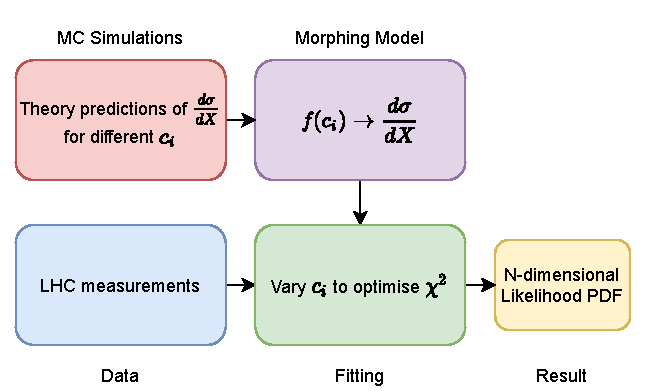
\includegraphics[width=0.5\textwidth]{images/deft-workflow.pdf}
    \caption{Overview of dEFT workflow}
\end{figure}

\subsection{Model building}
dEFT creates predictions for the observables of interest for varying values of Wilson coefficients by constructing a morphing model.
A morphing model is a linear regression model which allows for the interpolation between different templates.
These templates are Monte Carlo predictions which are generated around the region of parameter space which would be relevant for some dataset.
For dEFT's application, cross sectional SMEFT predictions which are generated using a event generation framework are treated as templates.
These predictions must describe the relevant set of operators $O_{i}$ with varying Wilson Coefficients in order to produce a reliable model.
Using ($\ref{eq:smeft_cross_section}$), a linear model is constructed using these templates and produces a predictive model $\hat{\sigma}({C_i})$.
This model now allows for the prediction of some cross sectional observable for any values of Wilson coefficients pertaining to the relevant set of operators.
Due to the reliance on MC samples, the model is dependent on the ability to produce high quality SMEFT differential cross section predictions.

The model must be validated to ensure sensible predictions are being performed and the model predicitons can be considered reliable.
Additional Monte Carlo samples are generated at coefficient values between the templates used to create the model.
Theses differential cross section samples are then compared to the model predictions to ensure the predictions agree within a suitable error comparable to the statistical error on the Monte Carlo samples.
Unfortunately, due to validating using Monte Carlo samples, this method of validation is still vulnerable to issues which may arise from the modelling of the samples themselves.

\subsection{Fitting Method}\label{sec:fitting}
Once a model has been built, a fit to data is possible.
dEFT performs fitting using Monte Carlo Markov Chain (MCMC) methods which allow for estimation of the likelihood distributions of the Wilson Coefficients using prior assumptions about their possible values.
The fitting procedure uses \emph{emcee}~\cite{Foreman_Mackey_2013} as its MCMC implementation.
MCMC requires an estimation for the likelihood function $P(y | C_{i})$ which represents the probability of obtaining some data $y$ given a set of model parameters $C_{i}$.

A common log likelihood definition for binned data with Gaussian errors with the associated model $f$ is
\begin{equation}\label{eq:likelihood}
    P(y | C_{i}) \propto \ln\mathcal{L}(y | C_{i}) = -\sum\limits_{n} (y_{n} - f_{n}(C_{i})) V^{-1} (y_{n} - f_{n}(C_{i}))
\end{equation}
where $y_{n}$ is the binned cross sectional data, $V$ is the associated covariance matrix and $f_{n}(C_{i})$ is the morphing model prediction.
In order for an estimation for the posterior likelihood distribution $P(C_{i} | y)$ to be made, a prior distribution $P(C_{i})$ is required.
This takes the form of uniform distributions defined by some minimum and maximum for each $C_{i}$ parameter.
MCMC will systematically sample throughout $C_{i}$ space building an estimation for the posterior distribution $P(C_{i}|y)$.
Properties regarding $C_{i}$ can then be inferred.

Since MCMC methods are used, an approximations for the $C_{i}$ distributions is obtained rather than a single value with an associated uncertainty which is common from other likelihood maximisation methods.
This avoids the issue of finding a local maximisation which can be common due to the quadratic nature of the SMEFT model.

The estimation for the coefficient is extracted from the likelihood distributions by considering percentiles of the discrete MCMC sampler prediction of the marginalised distribution of each operator.
The 50\ts{th} percentile is attributed as the estimation for the coefficient with the 16\ts{th} and 84\ts{th} percentile forming a 68\% confidence interval about the estimate.
This estimate allows for asymmetrical errors which can describe the measurement more faithfully than considering just the mean and variance of the samples.

\todo{talk about Smefit methods}

\section{Analysis}
This analysis will examine the possibility of using double differential cross section measurements with respect to multiple in a SMEFT analysis.
The results will be compared to outcomes when considering a single differential cross section.
The main aim of a SMEFT analysis is to place constraints onto Wilson coefficients of SMEFT operators allowing us to investigate the potential occurrences of new interactions or modifications to SM interaction.
Double differential cross sections are of interest due to the possibility of simultaneously constraining multiple operators which may present as different modifications to observable cross section distributions.

The only SMEFT operators considered were $O_{tG}$ and $O_{tq}^{8}$ with corresponding Wilson coefficients $C_{tG}$ and $C_{tq}^8$.
For a full phenomelogical study, the entire set of relevant operators should be included but this would drastically increase the scale of computational processing.
The limited set of operators should still show the influences of changing from a single dimensional differential cross section to a multidimensional differential cross section.

This analysis will begin with the details of discussion of the ATLAS datasets and the Monte Carlo event generation needed to create the morphing models for performing the constraints on the Wilson coefficients.
This will move into applying this model and obtaining estimations for the distribution of the coefficients for both the single observable and the double observable.

\subsection{Discussion of Datasets}
This report will use differential cross section data of top pair production from the ATLAS experiment~\cite{ATLAS:2019hxz} at the CERN Large Hadron Collider.
The data used is publicly available through HEPData~\cite{hepdata1750330}.
This data was produced from pp collisions performed at a centre-of-mass energy $\sqrt{s} = 13$TeV over the course of 2015 and 2016 with an integrated luminosity of 36.1fb$^{-1}$.
The $t\bar{t}$ final states are extracted from the $\ell$+jets channel in the resolved topology.
Resolved topology implies that the decay products of the hadronically decaying top quark are angularly well separated.

The double differential cross section observable considered  were the differential cross section as a function of the invariant mass of the $t\bar{t}$ system $m_{t\bar{t}}$ and the transverse momentum of the hadronically decaying top quark $p_{T}^{t}$.
These are the mass of the top-antitop system in it's rest frame and the component of the hadronically decaying top's momentum travelling radially from the beam line in the collider.
For the comparison with a single observable, the differential cross section as a function of just $m_{t\bar{t}}$ was examined.

The data provided contains the associated statistical and systematic uncertainties introduced during the measurements of the cross sections.
Multiple sources of systematic uncertainty are introduced in the process of measuring the $t\bar{t}$ systems.
This includes the uncertainty associated with the reconstruction of the lepton and the various jet products of the process.
There are also the uncertainty associated with the tagging of jets containing $b$-hadrons as well as accounting for possible misidentifications of jet flavour.
The uncertainty associated with the reconstruction of the missing transverse momentum $E_{T}^{\text{miss}}$ must also be accounted for.
Error in the modelling of the signal and background contributions and the Monte Carlo statistical error involved in creating these models are propagated.

Through HEPData, the covariance matrices associated with the differential cross section measurements are made available to the public.
The analysis was initially conducted including the full covariance matrix of each data set which was implemented into the likelihood definition as seen in (\ref{eq:likelihood}).
Unfortunately, this caused the likelihood definition to produce fits which described the data very poorly compared to if only the diagonals of the matrices were considered.
For the differential cross section data with respect to $m_{t\bar{t}}$, the fit produced with the full covariance matrix had a corresponding $\chi^2$ per degree of freedom of 12.60 while this was reduce to 0.53 when only considering the diagonal elements.
The covariance matrices provided were examined and it was found that they indicated that each bin in the histogram was highly correlated for a dataset of this type.
The single differential cross section histogram is shown as an example in Figure~\ref{fig:correlation}.
This was considered to be an error in the covariance matrix provided by HEPData and the covariance between different bins is ignored.

\begin{figure}[htb]
    \centering
    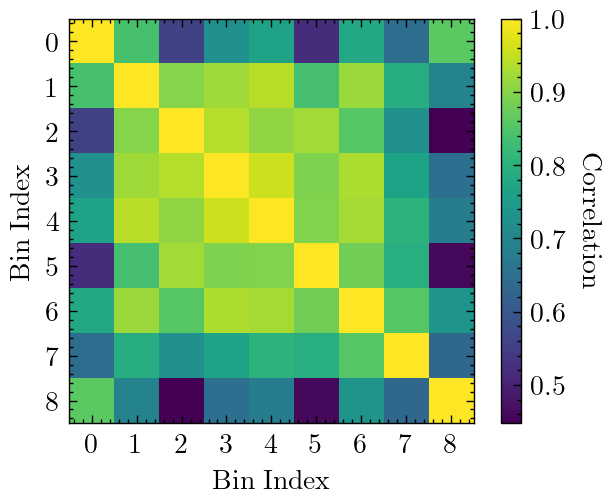
\includegraphics[width=0.5\textwidth]{plots/correlation.png}
    \caption{Correlation between $m_{t\bar{t}}$ bins of histogram for the differential cross section with respect to $m_{t\bar{t}}$ dataset}
    \label{fig:correlation}
\end{figure}



\todo{ask james about multiple smeft operators}


\subsection{Monte Carlo event generation}
In order to build the morphing model required to generate cross sectional predictions, simulated samples are required throughout the space of Wilson coefficients of the operators of interest.
These samples were generate using the MadGraph5\textunderscore aMC@NLO~\cite{Alwall_2014} framework which allows for the simulation of processes for a user-defined Lagrangian.
The SMEFTatNLO~\cite{degrande2020automated} FEYNRULES model implements SMEFT tree level and one loop processes into MadGraph5.
Though there is the capacity to perform predictions at next-to-leading order, these calculations are very recent \todo{Justify why LO better} and greatly increase the processing time required to produce the Monte Carlo predictions.
The simulations are performed to fixed order where only the desired observables of $m_{t\bar{t}}$ and ${p_{T}^{t}}$ are calculated and binned in the same binning arrangement as the ATLAS dataset of interest.

Separate sets of MC signal was required for the single observable and the double observables analysis.
Events were generated with values of $C_{tg}$ as -4, -3, -2.5, -2, -1, -0.5, 0, 0.5, 1, 2, 2.5, 3 and 4 and values of $C_{tq}^{8}$ as -4, -3, -2.5, -2, -1, -0.5, 0, 0.5, 1, 2, 2.5, 3 and 4. \todo{maybe rephrase this}
All permutations of these values were used resulting in a total number of 169 samples to build the model.
The model validation involved generating 100 validation samples at points different to those used for the building of the model.
This simulation step imposes a great challenge when wanting to expand into using more SMEFT operators in the model.
The number of required MC samples to ensure consistent description of the parameter space increases exponentially with the number of operators.
This is a major factor in the decision to not include all 4-fermion operators in this report and would require more time and computational capacity.
\todo{mention this fact in conclusion}

\subsubsection{Uncertainty due to simulation}

The simulation calculations were required to obtain a statistical accuracy of 1\% for the prediction of the integrated cross section of top-antitop production.
This level was considered a reliable since this error was minimal in comparison to the total uncertainty of the cross sectional data but still able to be performed in a reasonable time frame.
An accuracy requirement on each bin was unavailable and would have allowed for a clearer comparison to the error associated with the data.

Theoretical uncertainties on the Monte Carlo samples also needs to be accounted for.
This was done by varying the renormalisation and factorisation scales by two for the upper scale and by a half for the lower scale.
The scale variance was calculated through MadGraph5 using the SMEFTatNLO model with all operators being suppress.
This provided a scale variance prediction for the Standard Model at LO which could then be applied to SMEFT samples.
\todo{talk about error compared to validation value}
\todo{Maybe add plot comparing stat to mc error}
\todo{ask james about explaining scale variance}

\subsubsection{Calculation of \texorpdfstring{$k$}{k}-factor}
Since the generated Monte Carlo samples only included LO processes, theses predictions needed to be scaled to be comparable to the necessary data sets.
It can be considered fairly accurate to compare NNLO predictions to actual cross sectional data so a method of scaling the current predictions to this level is required.
Due to the difficulty in calculating the $k$-factor for different combinations of Wilson coefficients values, the $k$-factor for the Standard Model prediction was used across the various SMEFT predictions.

A flat $k$-factor across the differential cross sections was attempted to bring the LO predictions to the scale of NNLO predictions using the proportions between tree level calculations of total cross section~\cite{Alwall_2014} and measurement of total cross section using the ATLAS detector~\cite{ATLAS:2019hxz}.
This method failed due to some regions of the differential cross sections being poorly described at LO which caused a flat scaling to incorrectly describe the shape of the distributions at NNLO.
This is exemplified by the low $m_{t\bar{t}}$ and high $p_{T}^{t}$ region in our two observable data set, as seen in Figure~\ref{fig:kfactor}.
This is remedied by requiring a per-bin $k$-factor when scaling from LO to NLO but still using the flat factor to build up to NNLO.
The per-bin $k$-factor was found by comparing the Standard Model predictions of MadGraph5 at LO and NLO and applying this ratio to the Monte Carlo signal.
The theoretical error associated with the calculated $k$-factor is fairly difficult to propagate through the model construction and should be dominated by the error associated with the data.
This may have consequences on bins which are not well described at LO though the scale variances in these regions should dominate the uncertainties introduced by the $k$-factor.

\begin{figure}[H]
    \centering
    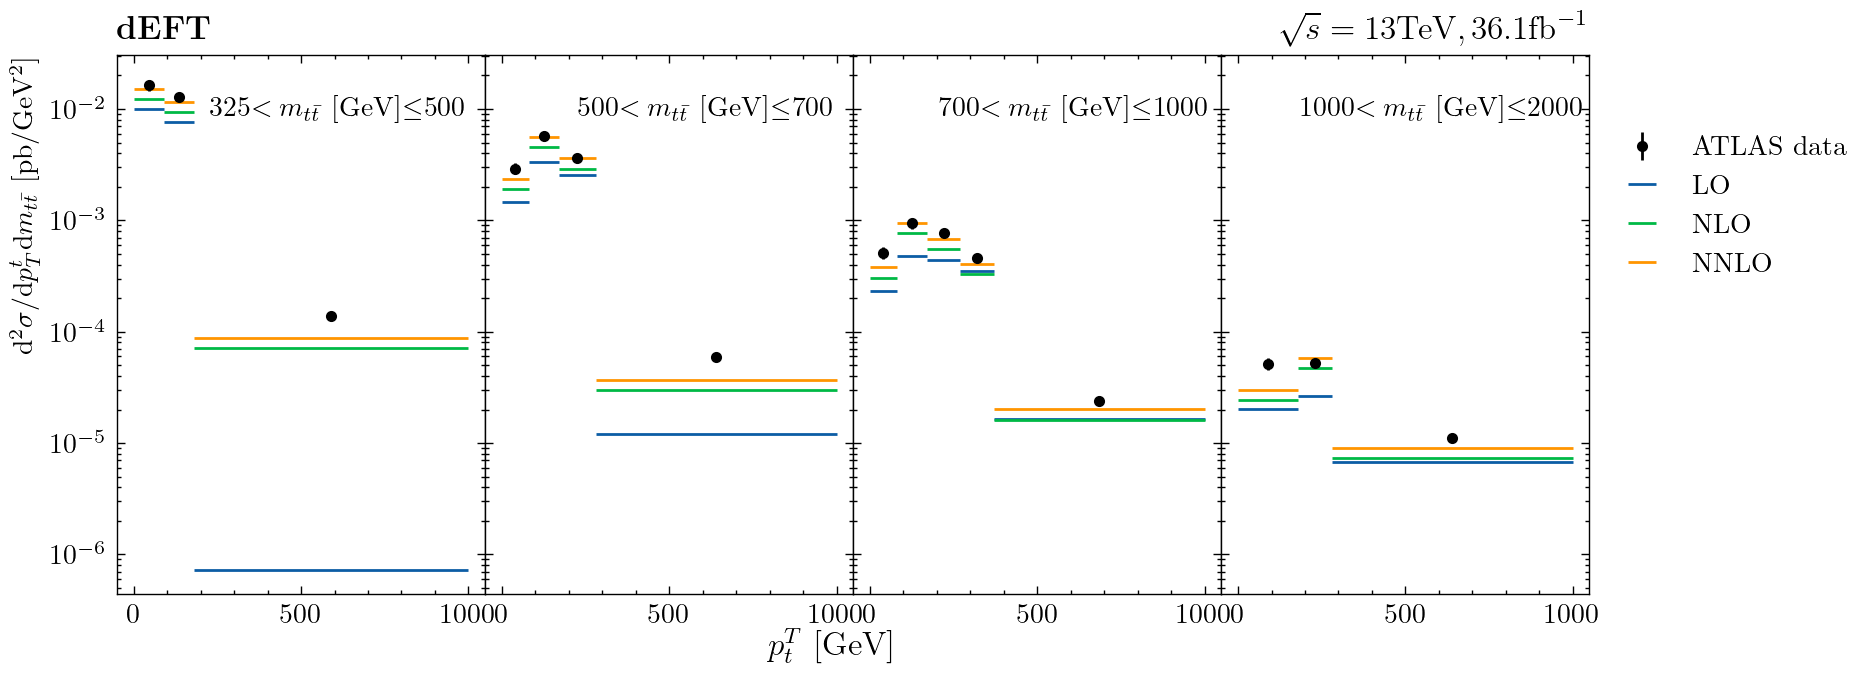
\includegraphics[width=0.8\textwidth]{plots/k_factor.png}
    \caption{Comparison of approximations for processes contributing to absolute double differential $t\bar{t}$ cross section with respect to $m_{t\bar{t}}$ and $p_{T}^{t}$. The scaling from an LO approximation to an NLO approximation was determined using a per-bin method and the NNLO prediction was determined using a flat factor.}
    \label{fig:kfactor}
\end{figure}


\subsection{\texorpdfstring{$m_{t\bar{t}}$}{mttbar} differential cross section}
\todo{Probably add an intro to the data set}
\todo{maybe add hepdata entry}
\todo{talk about covariance matrix}

\subsubsection{Model Validation}

The results of the validation testing can be seen in Figure~\ref{fig:residuals_hist_1D} where deviations between the model predictions and the validation samples are shown by the average relative residuals.
This deviation is expected to be comparable to the 1\% required accuracy for integrated cross section imposed on the event generation.
These tests appears to follow an accuracy of 1.09\% which is in-line with the expectation from the event generation.

\begin{figure}[htb]
    \centering
    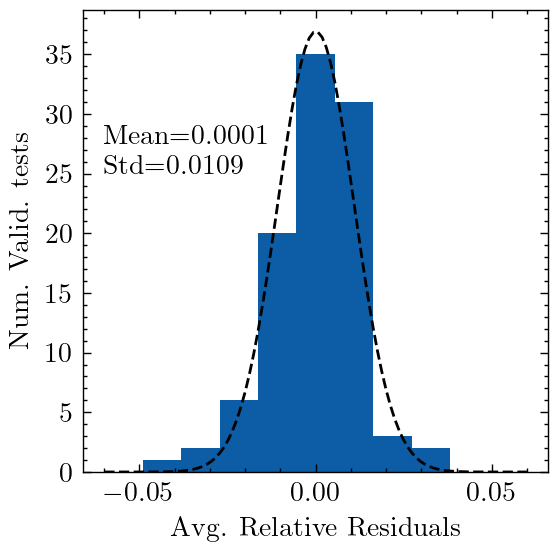
\includegraphics[width=0.4\textwidth]{./plots/residuals_hist_1D.png}
    \caption{Distribution of average relative residuals between model predictions at some set of coefficient values and the corresponding MC validation sample for the single observable model. This includes the validation tests over 100 different validation points. The dotted line represents a Gaussian fit to the histogram through $\chi^2$ minimisation with the results of the fit shown.}
    \label{fig:residuals_hist_1D}
\end{figure}
\todo{maybe include example validation plots}
\subsubsection{Results}

The estimations for the likelihood distributions for the Wilson coefficients are shown in Figure~\ref{fig:corner_1D_2OP}.
These distributions provide estimates $C_{tG}=0.24^{+0.11}_{-0.11}$ and $C_{tq}^{8}=1.56^{+0.25}_{-0.31}$ with theses estimates only considering statistical deviation of the distribution.
A notable features of the distribution is the second less prominent peak.
This is a product of the quadratic nature of the SMEFT model and shows that an alternative solution could still describe the data well.
The major peak in the distribution appears to show a slight correlation in the coefficients.

\begin{figure}[htb]
    \centering
    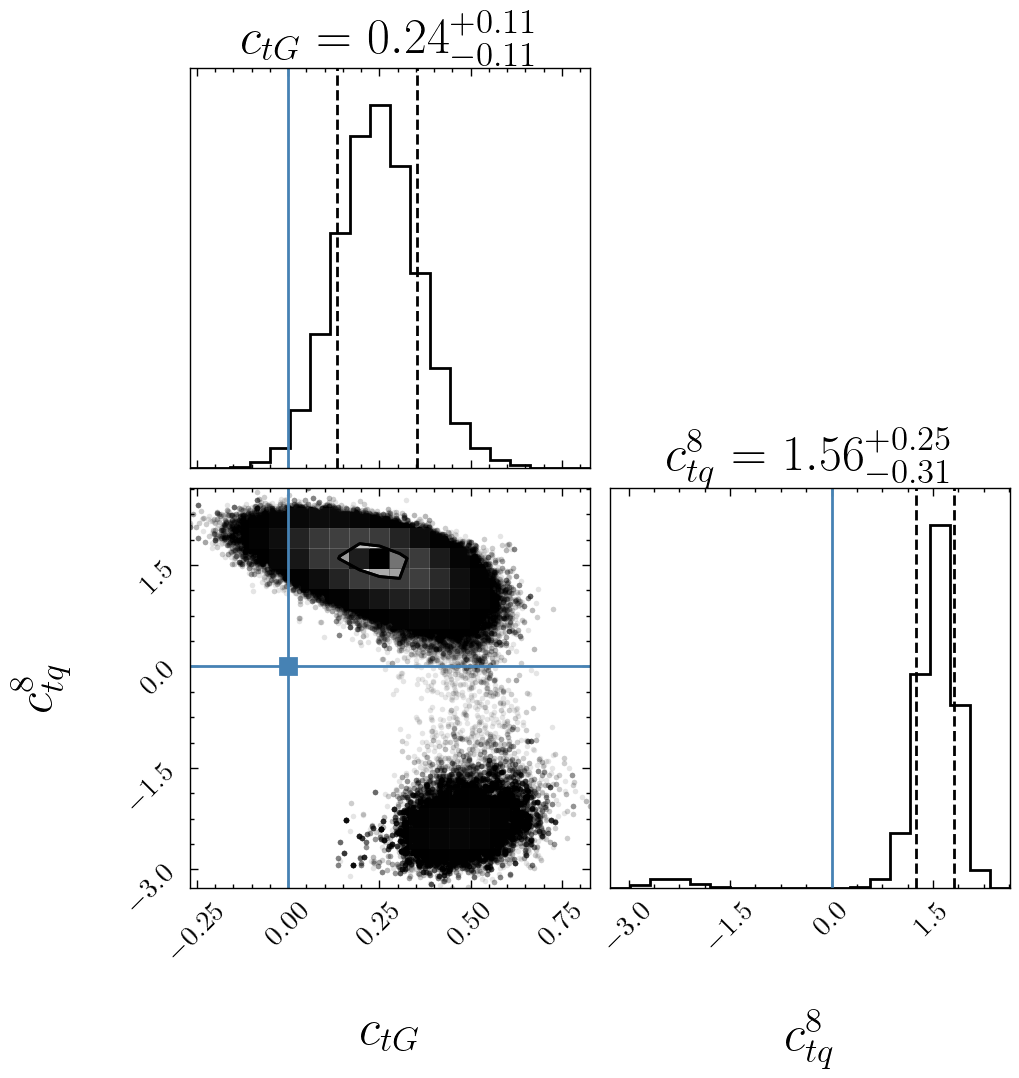
\includegraphics[width=0.4\textwidth]{plots/ATLAS-ctg-ctq8_1D_2OP.png}
    \caption{Estimation for the 2-dimensional likelihood distribution and 1-dimensional marginal distributions for the Wilson coefficient $C_{tG}$ and $C_{tq}^{8}$. The blue lines represent SM predictions. The dotted lines on the marginal distributions represent a 68\% confidence interval. Uncertainty estimates for the Wilson coefficients are the discussed in Section \ref{sec:fitting} and only represent statistical error.}
    \label{fig:corner_1D_2OP}
\end{figure}

The model created using the upper bound of the scale variance of the MC signal produced an estimation of $C_{tG}=0.22^{+0.12}_{+0.11}$ and $C_{tq}=1.39_{-0.35}^{+0.26}$.
The lower bound of the scale variance of the MC signal produced an estimation of $C_{tG}=0.26^{+0.11}_{0.11}$ and $C_{tq}=1.73_{-0.28}^{+0.24}$.
This implies a resulting systematic uncertainties introduced due to the scale variance of the simulated data of $\pm0.02$ for $C_{tG}$ and $\pm0.17$ for $C_{tq}^{8}$.

The single observable analysis obtained an estimate for the Wilson coefficients of $C_{tg} = 0.24 \pm 0.11 (stat.) \pm 0.02 (sys.)$ and $C_{tq}^{8}=1.56^{+0.25}_{-0.31} (stat.) \pm 0.17 (sys.)$.
The model prediction for this estimation can be seen in Figure~\ref{fig:model_result_1D_2OP}.
The predictions from the model at the optimised coefficients appears to better describe the data compared to using the model with all coefficients force to zero.
The optimised prediction corresponded to a $\chi^{2}$ per degree of freedom of 0.54 with respect to the data while the all zero prediction corresponded to a $\chi^{2}$ per degree of freedom of 3.16 indicating that the optimised prediction better describes the data.

\todo{talk to jame: is it close to zero}
The values obtained for the Wilson coefficients $C_{tG}$ and $C_{tq}^{8}$ seem to deviate from their Standard Model value of zero but still agree within 2 or 3 times the 68\% confidence interval.
This does provide some interest in possibly applying constraints beyond the Standard Model but there are some faults with this consideration.
The systematic uncertainty associated with the model creation and prediction was not accounted for in the uncertainty estimation.
Since these influences will equally be present when considering the double differential cross section data, this discussion will be deferred for later\todo{do the later} and these results will be used as a point of comparison between single and double observables analyses.


\begin{figure}[htb]
    \centering
    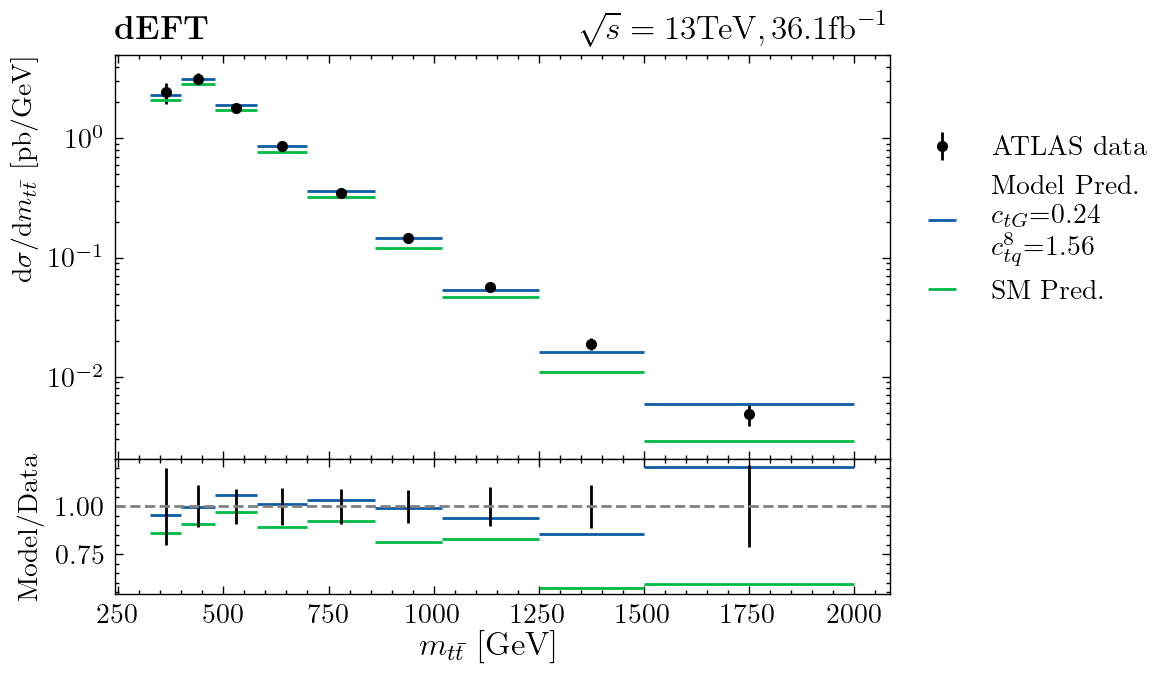
\includegraphics[width=0.6\textwidth]{plots/ATLAS_model_result_1D_2OP.png}
    \caption{Comparison of differential cross section of $t\bar{t}$ production as a function of $m_{t\bar{t}}$ between various morphing model predictions and ATLAS data. This includes model predictions for the optimised Wilson coefficients and for the all zero coefficient case (labelled as SM pred.). The ratio between each model prediction and the data is shown underneath. The errors shown represent statistical and systematic uncertainties of the data.}
    \label{fig:model_result_1D_2OP}
\end{figure}


\subsection{Double differential cross section}
\subsubsection{Model Validation}
The outcome of the validation tests of the double observable model are shown in Figure~\ref{fig:residuals_hist_2D}.
The average relative residuals appear to be distributed by a normal distribution with a deviation of 1.68\%.
This result is larger than the validation deviation of the single obervable but is still comparable to the statistical accuracy of the MC samples.


\begin{figure}[htb]
    \centering
    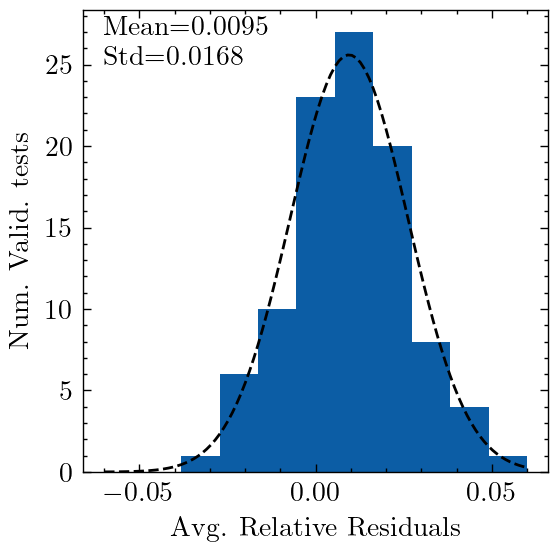
\includegraphics[width=0.4\textwidth]{plots/residuals_hist_2D.png}
    \caption{Distribution of average relative residuals between model predictions at some set of coefficient values and the corresponding MC validation sample for the double observable model. This includes the validation tests over 100 different validation points. The dotted line represents a Gaussian fit to the histogram through $\chi^2$ minimisation with the results of the fit shown.}
    \label{fig:residuals_hist_2D}
\end{figure}

\subsubsection{Results}

The estimations for the likelihood distributions for the Wilson coefficients are shown in Figure~\ref{fig:corner_2D_2OP}.
The distributions produced throught the MCMC method have estimates of the Wilson coefficient values of $C_{tG}=0.49_{-0.07}^{+0.06}$ and $C_{tq}^{8}=-0.51_{-0.70}^{+0.69}$.
The estimated systematic uncertainty associated with the scale variance of the simulated samples is $^{+0.11}_{-0.13}$ for $C_{tG}$ and $^{+0.21}_{-0.87}$ for $C_{tq}^{8}$. \todo{maybe change to table}
The final estimation for the Wilson coefficients are $C_{tG} = 0.49_{-0.07}^{+0.06}(stat) ^{+0.11}_{-0.13} (sys.)$ and $C_{tq}^{8}=-0.51_{-0.70}^{+0.69} (stat.) ^{+0.21}_{-0.87} (sys.)$.
The model prediction for this estimation can be seen in Figure~\ref{fig:model_result_1D_2OP}.

The shape of the distribution shows a more prominent double peak structure compared to what was seen in the single operator analysis.
This makes interpreting the value of the coefficients fairly difficult. \todo{more detail}

\begin{figure}[htb]
    \centering
    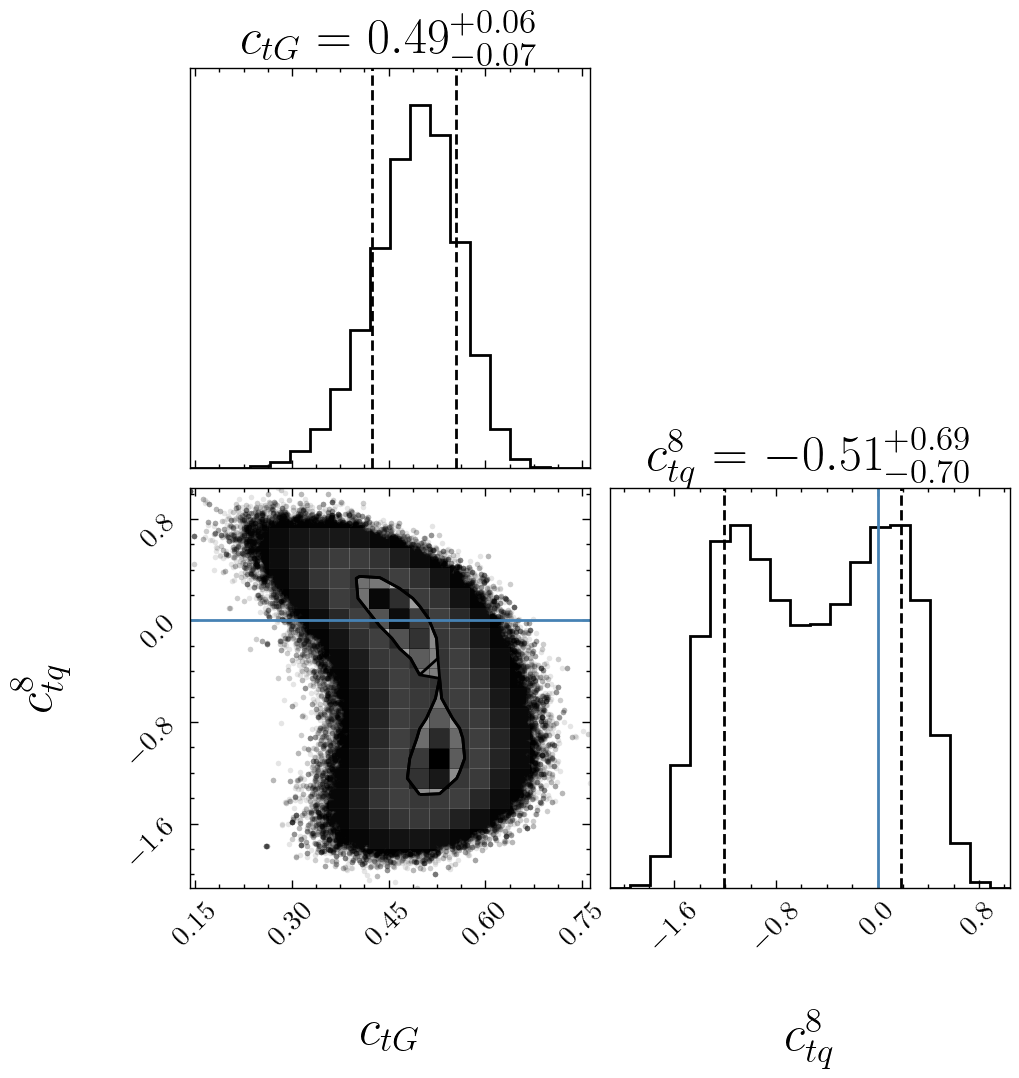
\includegraphics[width=0.4\textwidth]{plots/ATLAS-ctg-ctq8_2D_2OP.png}
    \caption{Estimation for the 2-dimensional likelihood distribution and 1-dimensional marginal distributions for the Wilson coefficient $C_{tG}$ and $C_{tq}^{8}$. The blue lines represent SM predictions. The dotted lines on the marginal distributions represent a 68\% confidence interval. Uncertainty estimates for the Wilson coefficients are the discussed in Section \ref{sec:fitting} and only represent statistical error.}
    \label{fig:corner_2D_2OP}
\end{figure}


\begin{figure}[htb]
    \centering
    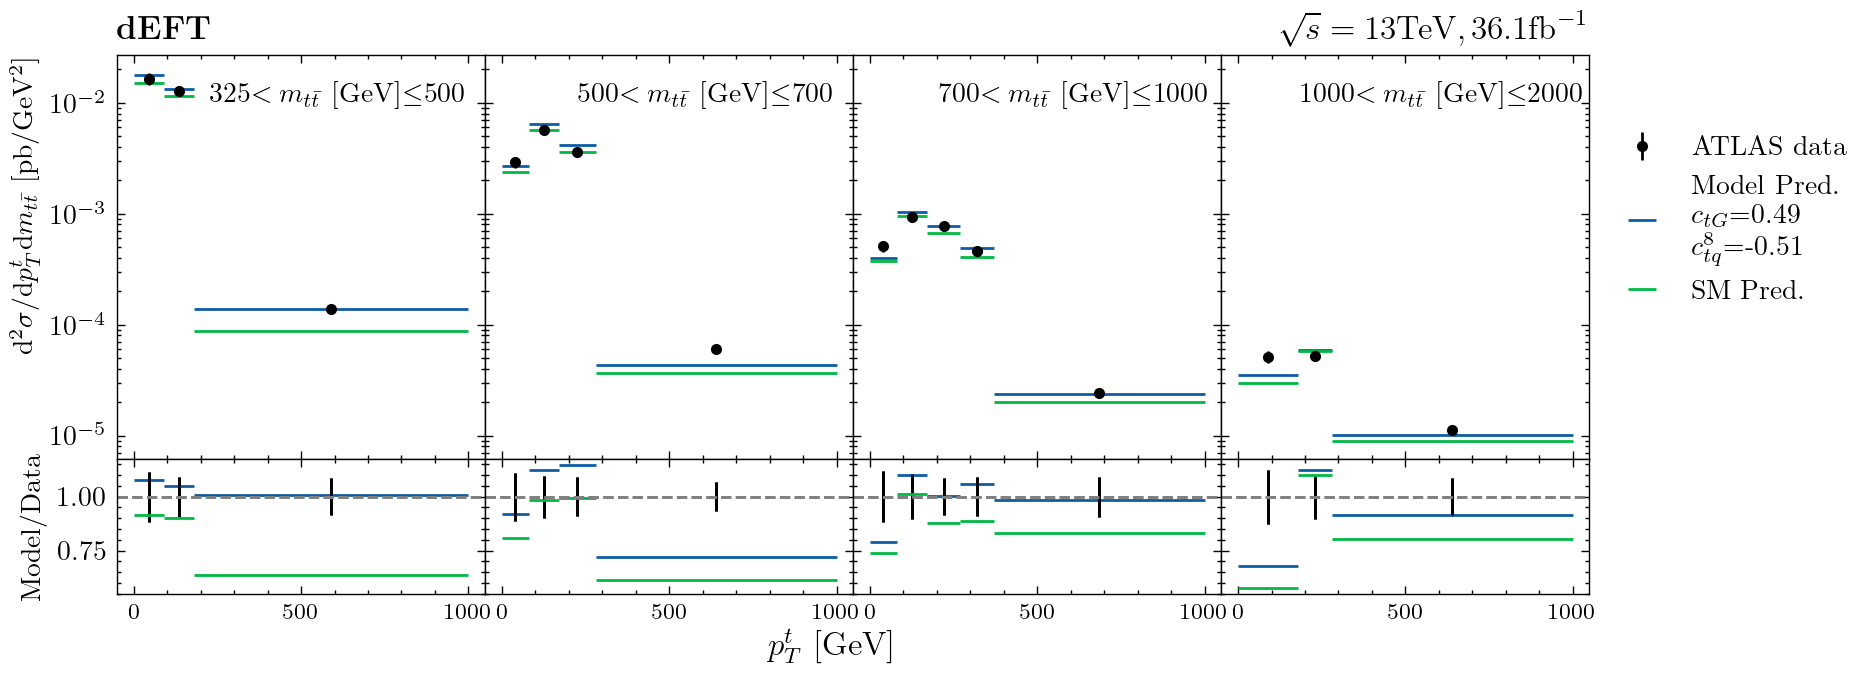
\includegraphics[width=0.8\textwidth]{plots/ATLAS_model_result_2D_2OP.png}
    \caption{Comparison of differential cross section of $t\bar{t}$ production as a function of $m_{t\bar{t}}$ and $p_{T}^{t}$ between various morphing model predictions and ATLAS data. This includes model predictions for the optimised Wilson coefficients and for the all zero coefficient case (labelled as SM pred.). The ratio between each model prediction and the data is shown underneath. The errors shown represent statistical and systematic uncertainties of the data.}
    \label{fig:model_result_2D_2OP}
\end{figure}

\section{Conclusion}

\clearpage
\begingroup
\raggedright{}
\sloppy
\printbibliography{}
\endgroup

\end{document}
